% ----- CHAPTER 3: NOTATION, DEFINITIONS AND BACKGROUND ----- %

%%%%%%%%%%%%%%%%%%%%%%%%%%
\section{Notation}\label{subsec:notation}

For the rest of the body of this text (unless otherwise stated) we set the following notation:
\begin{itemize}
\item $E$ is an elliptic curve over $\QQ$ given by minimal Weierstrass equation $y^2 + a_1 xy + a_3 y^2 = x^3 + a_2 x^2 + a_4 x + a_6$, where $a_1, a_3 \in \set{0,1}$, $a_2 \in \set{-1,0,1}$ and $a_4,a_6 \in \ZZ$
\item $D(E)$, $N(E)$ and $r_{al}(E)$  and $r_{an}(E)$ are the discriminant, conductor, algebraic rank and analytic rank of $E$ respectively. For ease of exposition, the dependence on $E$ will often be indicated by a subscript $E$ instead, and when there is no ambiguity it may be dropped entirely. Also, since much of this body of work assumes the validity of the the BSD conjecture, the algebraic and analytic rank of a curve will most often be assumed to be equal, in which case it will just be denoted $r_E$.
\item $p$ is a (rational) prime number and $q$ is a prime power
\item $s$ and $z$ are generic complex numbers
\item $L(E,s)$ and $\Lambda(E,s)$ are the standard and completed $L$-functions attached to $E$ respectively. Again, for ease of exposition we will in general subsume the $E$ into a subscript and write $\Les$ and $\Lams$.
\item $C(E) = C_E$ is the leading nonzero coefficient of the Taylor series of $\Lambda_E(s)$ about $s=1$.
\item $\gamma$ will always be used to denote the imaginary parts of nontrivial zeros of an $L$-function.
\item $\beta(E) = B_E$ is the bite of $E$, defined as $\beta_E = \sum_{\gamma\ne 0} \gamma^{-2}$, where $\gamma$ ranges over the noncentral nontrivial zeros of $\Les$
\item $\eta$ is the Euler-Mascheroni constant $= 0.5772156649\ldots$ \\
\end{itemize}

Furthermore, we define the following values associated to $E$ (in all cases the dependence on $E$ is understood):
\begin{itemize}
\item $b_2 = a_1^2 + 4a_2$
\item $b_4 = a_1 a_3 + 2a_4$
\item $b_6 = a_3^2 + 4a^6$
\item $b_8 = a_1^2 a_6 + 4 a_2 a_6 - a_1 a_3 a_4 + a_2 a_3^2 - a_4^2$
\item $c_4 = b_2^2 - 24 b_4$
\item $c_6 = -b_2^3 + 36 b_2 b_4  - 216 b_6$
\item $D = D_E = -b_2^2 b_8 - 8 b_4^3 - 27 b_6^2 + 9 b_2 b_4 b_6$; this is the definition of the discriminant of $E$
\item $j = \frac{c_4}{D}$ is the $j$-invariant of $E$
%\item $\omega = \frac{dx}{2y + a_1 x + a_3} = \frac{dy}{3x^2 + 2a_2 x + a_4 - a_1 y}$
\end{itemize}

\newpage
%%%%%%%%%%%%%%%%%%%%%%%%%%
\section{Definitions and Basic Results}

The rest of this chapter covers the basic definitions of and results needed for the rest of this work (namely, big-Oh notation, elliptic curves and $L$-functions). Feel free to skip this if you are familiar with them.

%%%%%%%%%%%%
\subsection{Big-Oh Notation}

Given that the running time of various algorithms will be discussed over the course of this work, we recall the definitions of big-Oh and soft-Oh notation, at least in the context of how they will be used here.

\begin{definition}
Let $x$ be a positive input, and let $g(x)$ be some positive-valued reference function on $x$.
\begin{itemize}
\item We say a function $f(x) = O(g(x))$ (read ``$f$ is big-Oh of $g$''), if
\begin{equation}
\limsup_{x \to \infty} \left| \frac{f(x)}{g(x)}\right| < \infty
\end{equation}
That is, $f(x) = O(g(x))$ if the asymptotic growth/decay rate of $f$ is bounded by some multiple of that of $g$.
\item We say a function $f(x) = \softO(g(x))$ (read ``$f$ is soft-Oh of $g$''), if there is some $k>0$ such that
\begin{equation}
\limsup_{x \to \infty} \left| \frac{f(x)}{g(x)\left(\log g(x)\right)^k}\right| < \infty
\end{equation}
That is, $f(x) = \softO(g(x))$ if the asymptotic growth/decay rate of $f$ scales like that of $g$, up to the inclusion of log factors.
\end{itemize}
\end{definition}
Note that $f(x) = \softO(g(x))$ is equivalent to the statement that $f(x) = O(g(x)^{1+\epsilon})$ for any $\epsilon>0$. \\

\begin{definition}
Let $A$ be an algorithm which takes input $n$, where for simplicity we may think of $n$ as a positive integer. Let $t_A(n)$ be the running time of $A$ on the input $n$.
\begin{itemize}
\item $A$ is said to have {\it polynomial time complexity} if there is some $k>0$ such that the running time of $t_A(n) = O(n^{k})$, i.e. the asymptotic running time of the algorithm scales like some polynomial function of $n$.
\item If $t_A(n) = O(n^{\epsilon})$ for any $\epsilon>0$, then $A$ is said to have {\it sub-polynomial time complexity}. Note that if $t_A(n) = \softO(1)$, then $A$ has sub-polynomial time complexity.
\item If no $k>0$ exists such that $t_A(n) = O(n^k)$, then $A$ is said to have {\it super-polynomial time complexity}. More specifically, if there is some $k>1$ such that $t_A(n) = O(k^n)$, then $A$ is said to have {\it exponential time complexity}.
\end{itemize}
\end{definition}
The same terminology can be applied to the space requirements of an algorithm, wherein we would replace the word `time' with `space'.


%%%%%%%%%%%%
\subsection{Elliptic curves}

\begin{definition}
An elliptic curve $E$ is a genus 1 smooth projective curve with a marked point $\cO$. $E$ is defined over a field $K$ if $E$ may be represented by the {\it Weierstrass equation} $y^2 + a_1 xy + a_3 y^2 = x^3 + a_2 x^2 + a_4 x + a_6$, where $a1,\ldots a_6 \in K$.
\end{definition}

For elliptic curves defined over $\QQ$, we may always find a model for $E$ such that $a_1, a_3 \in \set{0,1}$, $a_2 \in \set{-1,0,1}$ and $a_4,a_6 \in \ZZ$. Furthermore, there is the notion of {\it minimality} when it comes to models for elliptic curves. Without going into the definition thereof, unless stated otherwise we will assume that any given elliptic curve Weierstrass equation is minimal and in the above form.

\begin{definition}
The set of $K$-rational points on $E$ is denoted $E(K)$. $E(K)$ comprises an abelian group, with the ``point at infinity" $\cO$ acting as the group identity element.
\end{definition}

It is often useful to view an elliptic curve $E$ as the vanishing locus of the polynomial
\begin{equation}\label{eqn:E_poly}
f(x,y) = y^2 + a_1 xy + a_3 y^2 - x^3 - a_2 x^2 - a_4 x - a_6.
\end{equation}
 That is $E(K) = \set{(x,y) \in K^2: \; f(x,y) = 0}$, along with the point at infinity $\cO$. \\

For a rational elliptic curve $E/\QQ$, we may consider the reduced curve $\tilde{E}/\Fp$ for any prime $p$. If $E/\QQ$ is given by $y^2 + a_1 xy + a_3 y^2 = x^3 + a_2 x^2 + a_4 x + a_6$, then for $p\ne 2$ or $3$ the reduced curve is given by $y^2 + \overline{a_1} xy + \overline{a_3} y^2 = x^3 + \overline{a_2} x^2 + \overline{a_4} x + \overline{a_6}$, where $\overline{a_i}$ is $a_i$ reduced modulo $p$. For $p = 2$ or $3$ we may have to move to a different model for $E$ first to avoid the reduced curve being automatically singular.

\begin{definition}
A prime $p$ is called {\it good} if $\tilde{E}/\Fp$ is non-singular. The reduced curve is an elliptic curve over $\Fp$ (by definition) which we denote by $E/\Fp$; $E$ is said to have {\it good reduction at $p$}. Otherwise, $p$ is said to be {\it bad}, the reduced (singular) curve is denoted $\tilde{E}/\Fp$, and $E$ is said to have {\it bad reduction at $p$}.
\end{definition}

\begin{theorem}
For any $E/\QQ$, the set of bad primes is finite and non-empty.
\end{theorem}

Singular reduced curves may be thought of as finite-field analogues of singular cubics over the rationals, for example those given by $y^2 = x^3$ and $y^2 = x^3+x^2$ as seen below. Singular curves have a (unique) {\it singular point}, which is by definition where the partial derivatives $\frac{\partial f}{\partial x}$ and $\frac{\partial f}{\partial y}$ are both zero (here $f$ is as given by equation \ref{eqn:E_poly}).

\begin{figure}[!h]
    \centering
    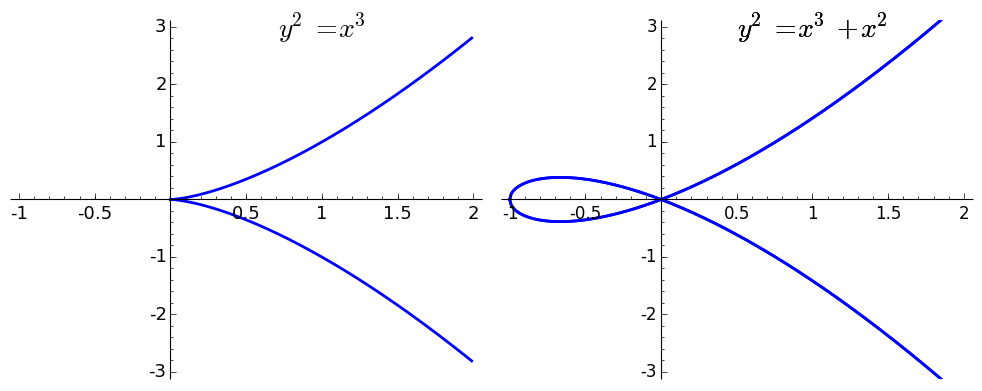
\includegraphics[width=1.0\textwidth]{graphics/singular_cubics.png}
    \caption{An example of two singular cubics over the rationals. The singular point for both curves is at the origin; for the the left curve the singular point is a {\it cusp}, and for the right curve it is a {\it node}.}
    \label{fig:singular_cubics}
\end{figure}

In the finite field setting the notion of partial derivatives still makes sense, so one may define singular points accordingly. Bad reduction at a prime may be classified into one of three types according to the nature of the tangent space at the singular point on $\tilde{E}/\Fp$.
\begin{definition}
Let $E$ have bad reduction at $p$; let $P$ be the singular point on $\tilde{E}/\Fp$, and let $T_P(E)$ be the tangent space at $P$.
\begin{itemize}
\item If the $T_P(E)$ is one-dimensional, then $P$ is a cusp, and $E$ is said to have {\it additive reduction} at $p$.
\item Otherwise $T_P(E)$ is two-dimensional, and $P$ is then a node; $E$ is then said to have {\it multiplicative reduction} at $p$. Furthermore, multiplicative reduction can be decomposed into two cases:
\begin{itemize}
\item If $T_P(E)$ is defined over $\Fp$, then $E$ is said to have {\it split multiplicative reduction} at $p$
\item Otherwise $T_P(E)$ is defined over a quadratic extension of $\Fp$, and $E$ is said to have {\it non-split multiplicative reduction} at $p$.
\end{itemize}
\end{itemize}
\end{definition}

Primes of bad reduction are packaged together into an invariant called the {\it conductor} of $E$:
\begin{definition}
The conductor of $E$, denoted by $N_E$, is a positive integer given by
\begin{equation}
N_E = \prod_{p} p^{f_p(E)},
\end{equation}
where $p$ ranges over all primes, and for $p \ne 2$ or $3$,
\begin{equation}
f_p(E) = \begin{cases} 0, & \text{$E$ has good reduction at $p$} \\ 1, & \text{$E$ has multiplicative reduction at $p$} \\ 2, & \text{$E$ has additive reduction at $p$.}\end{cases}
\end{equation}
For $p=2$ and $3$, the exponent $f_p(E)$ is still zero if $p$ is good; however the exponent may be as large as $8$ and $5$ respectively if $p$ is bad.
\end{definition}
The ``proper" definition of the conductor is Galois representation-theoretic and is defined in terms of the representation of the inertia group at $p$ on the torsion subgroup of $E$; For $p\ne 2$ or $3$ this reduces to the definition given above, but for $2$ and $3$ there may be nontrivial wild ramification which increases the exponent up to the stated amounts. A full technical definition of the conductor is given in \cite[pp. 379-396]{Sil-1994}. In any case (including $2$ and $3$), the exponent $f_p(E)$ may be computed efficiently by Tate's algorithm, as detailed in the previous section of the same book \cite[pp. 361-379]{Sil-1994}. \\

%%%%%%%%%%%%
\subsection{Elliptic curve $L$-functions}

We now move on to the definition of the $L$-function attached to an elliptic curve. For this we must define the numbers $a_p(E)$:
\begin{definition}\label{def:a_p} \mbox{}
\begin{itemize}
\item For good primes $p$ (i.e. when $p \nmid N_E$), let
\begin{equation}
a_p(E) = p+1-\#\set{\EFp},
\end{equation}
where $\#\set{\EFp}$ is the number of points on $E/\Fp$;
\item For bad primes (when $p \mid N_E$), let
\begin{equation}
a_p(E) := \begin{cases}
+1 & \text{if $E$ has split multiplicative reduction at $p$} \\
-1 & \text{if $E$ has non-split multiplicative reduction at $p$} \\
0 & \text{if $E$ has additive reduction at $p$.}
\end{cases}
\end{equation}
\end{itemize}
\end{definition}

Hasse's theorem states that the number of points on $E$ modulo $p$ can never be too far from $p+1$:
\begin{theorem}[Hasse, 1936]
For all elliptic curves $E/\QQ$ and all primes $p$,
\begin{equation}
|a_p(E)| \le \sqrt{p}
\end{equation}
\end{theorem}

For ease of notation, when $E$ is fixed we will let $a_p := a_p(E)$, letting the dependence on $E$ be understood. \\

The Sato-Tate Conjecture, now a theorem thanks to Taylor, goes even further, giving an asymptotic distribution on the $a_p$:
\begin{theorem}[Taylor, 2006-]
For fixed $E/\QQ$, the set of normalized $a_p$ values $\set{\frac{a_p}{2\sqrt{p}}: p \text{ prime}}$ obey a semicircular distribution on the interval $[-1,1]$. That is, for $1\le a \le b \le 1$, the asymptotic proportion of primes for which $a \le \frac{a_p}{2\sqrt{p}} \le b$ is equal to the proportion of the area under the unit semicircle between $a$ and $b$.
\end{theorem}

\begin{definition} \mbox{}

The $L$-function attached to $E$ is a complex analytic function $L_E(s)$, defined initially on some right half-plane of the complex plane.
\begin{itemize}
\item The Euler product of the $L$-function attached to $E$ is given by
\begin{equation}
L(E,s) = \prod_{p} \frac{1}{1 - a_p p^{-s} + \epsilon(p)p^{1-2s}}
\end{equation}
where $\epsilon(p) = 0$ for bad $p$, and $1$ for good $p$.
\item The Dirichlet series for $L_E(s)$ is given by
\begin{equation}
L(E,s) = \sum_{n=1}^{\infty} a_n n^{-s}.
\end{equation}
where for composite $n$, $a_n$ is defined to be the integer coefficient of $n^{-s}$ obtained by multiplying out the Euler product for $L(E,s)$.
\end{itemize}
\end{definition}
Again, we will often write $\Les$ or just $L(s)$ to simplify notation. \\

\begin{corollary} \mbox{}
\begin{itemize}
\item Hasse's Theorem implies that the Euler product and Dirichlet series for $\Les$ converge absolutely for $\Re(s) > \frac{3}{2}$.
\item Sato-Tate implies that the Euler product and Dirichlet series for $\Les$ converge conditionally for $\Re(s) > \frac{1}{2}$.
\end{itemize}
\end{corollary}

In this work we more often use the completed $L$-function attached to $E$:
\begin{definition}
The {\it completed $L$-function} attached to $E$ is given by
\begin{equation}
\Lambda_E(s) = (N_E)^{\frac{s}{2}}(2\pi)^{-s}\Gamma(s)\Les,
\end{equation}
where $N_E$ is the conductor of $E$ and $\Gamma(s)$ the usual Gamma function on $\CC$.
\end{definition}

Thanks to the modularity theorem, we may in fact analytically continue $\Les$ and $\Lams$ to be entire functions defined on all of $\CC$.
\begin{theorem}[Breuille, Conrad, Diamond, Taylor, Wiles et al, 1995,1999,2001] \mbox{}\\
There exists an integral newform $f = \sum_n a_n q^n$ of of weight $k=2$ and level $N_E$ such that $\Les = L_f(s)$.
\end{theorem}

The modularity theorem above is essentially the converse of the theorem by Shimura in the 1960s: if $f$ is a weight $2$ newform of level $N_E$, then there exists some elliptic curve $E/\Q$ of conductor $N_E$ such that $L_f(s) = L_E(s)$. Hence any theorem about elliptic curve $L$-functions is thus really a theorem about $L$-functions of weight 2 newforms in disguise. \\

\begin{corollary} \mbox{}
\begin{itemize}
\item $\Lams$ extends to an entire function on $\CC$. Specifically, $\Lams$ obeys the {\it functional equation}
\begin{equation}
\Lams = w_E \Lambda_E(2-s),
\end{equation}
where $w_E \in \set{-1, 1}$ is the action of the Atkin-Lehner involution on the newform attached to $E$.
\item $\Les$ extends to an entire function on $\CC$ via the definition of $\Lams$ and the functional equation above.
\end{itemize}
\end{corollary}

We reproduce the analytic continuation for $\Lams$ explicitly below. Define the auxiliary function $\lambda_E(s)$ by
\begin{equation}\label{eqn:Lams_analytic_continuation}
\lambda_E(s) = \left(\frac{\sqrt{N_E}}{2\pi}\right)^{s} \sum_{n=1}^\infty a_n n^{-s}\Gamma \left(s,\frac{2\pi n}{\sqrt{N_E}}\right),
\end{equation}
where all the quantities are as defined previously, and $\Gamma(s,x)$ is the upper incomplete Gamma function on $\CC\cross \RR_{>0}$. The sum converges absolutely for any $s$, so $\lambda_E(s)$ is entire. Then
\begin{equation}
\Lambda_E(s) = \lambda_E(s) + w_E \lambda_E(2-s)
\end{equation}
Knapp goes through the proof of this formula in \cite[pp. 270-271]{Kna-1992}. \\

\begin{definition}
$E$ is said to have {\it even parity} if $w_E = 1$, and {\it odd parity} if $w_E = -1$.
\end{definition}

The functional equation for $\Lams$ shows that it is either symmetric or antisymmetric about the line $\Re(s) = 1$; moreover, since all the constituent parts for $\Lams$ are defined over the reals, $\Lams$ is also conjugate symmetric about the real axis. It follows that $\Lams$ is highly symmetric about the point $s=1$. This is formalized in the following statement:
\begin{proposition}
As a function of $s$, $\Lambda_E(1+s)$ is even if $E$ has even parity, and odd if $E$ has odd parity.
\end{proposition}
This follows immediately from the functional equation. \\

\begin{definition} For elliptic curve $L$-functions:
\begin{itemize}
\item The point $s=1$ is called the {\it central point} or the {\it critical point}.
\item The vertical line of symmetry $\Re(s)=1$ is called the {\it critical line}.
\item The vertical strip $\frac{1}{2} \le \Re(s) \le \frac{3}{2}$ is call the {\it critical strip}.
\end{itemize}
\end{definition}

There is an oft-quoted anecdote that the way to differentiate analytic number theorists from algebraic number theorists is that for elliptic curve $L$-functions the former normalize so that the critical line lies at $\Re(s) = \frac{1}{2}$ (as is the case with $\zeta(s)$), while the latter keep the critical line at $\Re(s)=1$. In this thesis we work mostly with $L_E(1+s)$ and $\Lambda_E(1+s)$ which shifts the critical line to the imaginary axis; a move which is bound to antagonize both parties equally! \\

A standard result with $L$-functions of Hecke eigenforms (of elliptic curve $L$-functions are a subset) is that ``all the interesting stuff happens inside the critical strip'':
\begin{proposition}
For any $E/\QQ$,
\begin{equation}
\Lambda_E(1+s) \ne 0 \;\;\mbox{when}\;\; |\Re(s)| > \frac{1}{2}
\end{equation}
\end{proposition}
This can be proven by showing that the logarithmic derivative of $\Lambda_E(1+s)$ converges absolutely for $\Re(s) > \frac{1}{2}$; see the corollary to Proposition \ref{lem:ldLe_bound} for a proof. The statement can with a bit more work be strengthened to asserting that all zeros are {\it strictly} inside the critical strip). In fact, the Generalized Riemann Hypothesis asserts that
\begin{equation}
\Lambda_E(1+s) \ne  \;\;\mbox{when}\;\; \Re(s) \neq 0
\end{equation}
From the functional equation we get that $\Les$ has simple zeros at the nonpositive integers; these are denoted the {\it trivial} zeros of $\Les$. Zeros inside the critical strip are called {\it nontrivial}. The Generalized Riemann Hypothesis (stated in full in section \ref{sec:conjectures}) asserts that all nontrivial zeros of $\Les$ lie on the critical line $\Re(s)=1$, and all zeros with nonzero imaginary part are simple. 

If $\Les$ has a zero at the central point, it may or may not have multiplicity greater than 1. The multiplicity of this possible zero is denoted the analytic rank of $E$:
\begin{definition}
Let $E$ be an elliptic curve over $\Q$, and let $\Les$ be its $L$-series. The {\it analytic rank} of $E$, denoted $r_{an}(E)$ or just $r_{an}$ is the order of vanishing of $L_E(s)$ at the central point $s=1$. That is, if the Taylor series of $\Les$ about $s=1$ is
\begin{equation}
L_E(1+s) = a_0 + a_1 s + a_2 s^2 + \ldots
\end{equation}
then $a_n = 0$ for $0 \le n < r_{an}$ and $a_{r_{an}} \ne 0$.
\end{definition}
We will work a lot with the leading coefficient of the $L$-seres at the central point, so it's worth giving it a name. To this end:
\begin{definition} \mbox{}
\begin{itemize}
\item Let $C\pr_E$ (or just $C\pr$ when $E$ is fixed) be the leading coefficient of $L_E(s)$ at the central point (the constant $a_{r_{an}}$ in the definition above)
\item Let $C_E$ (or just $C$ when $E$ is fixed) be the leading coefficient of $\Lams$ at the central point.
\end{itemize}
\end{definition}
Observe that $C\pr_E = \frac{2\pi}{\sqrt{N_E}}\cdot C_E$. We will most often work with the latter, hence the notation. \\

We may use Equation \ref{eqn:Lams_analytic_continuation} to produce formulae for the value of $\Lams$ and its higher derivatives at the central point:
\begin{proposition} \mbox{}
\begin{enumerate}
\item \begin{equation}
\Lambda_E(1) = \begin{cases} \frac{\sqrt{N_E}}{\pi} \sum_{n=1}^{\infty}\frac{a_n}{n} e^{-\frac{2\pi}{\sqrt{N_E}}\cdot n}, & w_E = 1 \\ 0, & w_E = -1 \end{cases}
\end{equation}
\item When $m$ has the same parity as $E$, the $m$th derivative of $\Lams$ at the central point is given by
\begin{equation}\label{eqn:central_derivatives}
\Lambda_E^{(m)}(1) = 2 \sum_{n=1}^\infty a_n \int_{1}^{\infty} \left(\log \frac{t}{\sqrt{N_E}}\right)^m e^{-\frac{2\pi n}{\sqrt{N_E}}\cdot t} \; dx
\end{equation}
When $m$ is opposite in parity to $E$, then $\Lambda_E^{(m)}(1) = 0$.
\end{enumerate}
\end{proposition}

\begin{proof}
Observe we may write equation \ref{eqn:Lams_analytic_continuation}, after a change of variables and swapping integration and summation signs, as
\begin{equation*}
\lambda_E(1+s) = N_E^{\frac{1+s}{2}}  \int_{\frac{1}{\sqrt{N_E}}}^{\infty} x^s f_E(it) \; dt  = N_E^{\frac{1+s}{2}}  \sum_{n=1}^\infty a_n \int_{\frac{1}{\sqrt{N_E}}}^{\infty} t^s e^{-2\pi nt} \; dt,
\end{equation*}
where $f_E$ is the cusp form attached to $E$. We may differentiate under the integral sign without issue and then evaluate at $s=1$ to get
\begin{equation}\label{eqn:lambda_derivs}
\lambda_E^{(m)}(1) = \sqrt{N_E}\cdot \sum_{n=1}^\infty a_n \int_{\frac{1}{\sqrt{N_E}}}^{\infty} (\log t)^m e^{-2\pi n t} \; dt
\end{equation}
Equation \ref{eqn:central_derivatives} follows by substituting $t \mapsto \sqrt{N_E} \cdot t$. For $m=0$ the integrals may be evaluated directly: $\int_{1}^{\infty} e^{-\frac{2\pi n t}{\sqrt{N_E}}} \; dt = \frac{\sqrt{N_E}}{2\pi n} e^{-\frac{2\pi n}{\sqrt{N_E}}}$.
\end{proof}


Equation \ref{eqn:central_derivatives} allows us to establish bounds on the coefficients of the Taylor expansion of $\Lams$ about the central point. For this we will need the following technical lemma:
\begin{lemma}\label{lem:central_deriv_int_bounds}
Let $N_E,n \in \ZZ_{>0}$, and suppose $m$ is a positive integer such that $m < \frac{1}{2}\log N_E$. Then
\begin{equation}
\left| \int_{\frac{1}{\sqrt{N_E}}}^{\infty} (\log t)^{m} e^{-2\pi n t} \; dt \right| < \frac{\left(\frac{1}{2} \log N_E\right)^{m}}{2\pi n}\left[ e^{-\frac{2\pi n}{\sqrt{N_E}}} + \frac{e^{-2\pi n\sqrt{N_E}}}{2\pi n \sqrt N_E} \right].
\end{equation}
\end{lemma}
\begin{proof}
We split the integral in two, dealing with the intervals $\frac{1}{\sqrt{N_E}}$ to $\sqrt{N_E}$ and $\sqrt{N_E}$ to $\infty$ separately. Now $(\log t)^{m}$ is at most $(\frac{1}{2}\log N_E)^m$ in magnitude on $[\frac{1}{\sqrt{N_E}},\sqrt{N_E}]$, so
\begin{equation*}
\left| \int_{\frac{1}{\sqrt{N_E}}}^{\sqrt{N_E}} (\log t)^{m} e^{-2\pi n t} \; dt \right| < \left(\frac{1}{2} \log N_E\right)^m \int_{\frac{1}{\sqrt{N_E}}}^{\sqrt{N_E}} e^{-2\pi n t} \; dt < \frac{\left(\frac{1}{2} \log N_E\right)^{m}}{2\pi n}\left(e^{-\frac{2\pi n}{\sqrt{N_E}}} - e^{-2\pi n\sqrt{N_E}}\right)
\end{equation*}
For the integral on $[\sqrt{N_E},\infty)$, we use integration by parts to get
\begin{equation*}
\int_{\sqrt{N_E}}^{\infty} \left(\log t \right)^{m} e^{-2\pi n t} \; dt = \frac{\left(\frac{1}{2} \log N_E\right)^{m}}{2\pi n}\cdot e^{-2\pi n\sqrt{N_E}} + \frac{m}{2\pi n} \int_{\sqrt{N_E}}^{\infty} \frac{\left(\log t \right)^{m-1}}{t} e^{-2\pi n t} \; dt 
\end{equation*}
If $m < \frac{1}{2}\log N_E$, then $\frac{\left(\log t \right)^{m-1}}{t}$ is decreasing for $t > \sqrt{N_E}$, so we have
\begin{equation*}
\frac{m}{2\pi n} \int_{\sqrt{N_E}}^{\infty} \frac{\left(\log t \right)^{m-1}}{t} e^{-2\pi n t} \; dt < \frac{m\left(\frac{1}{2} \log N_E\right)^{m-1}}{2\pi n\sqrt{N_E}} \int_{\sqrt{N_E}}^{\infty} e^{-2\pi n t} \; dt < \frac{\left(\frac{1}{2} \log N_E\right)^{m}}{(2\pi n)^2 \sqrt{N_E}} \cdot e^{-2\pi n \sqrt{N_E}}.
\end{equation*}
Add up all the values and you get the established result.
\end{proof}

With the above lemma in hand, we establish an upper bound on the magnitude of the $m$th Taylor coefficient of $\Lams$ at the central point.
\begin{proposition}\label{prop:central_deriv_bounds}
Let $E$ have conductor $N_E$ and completed $L$-function $\Lams$. Then so long as $m<\frac{1}{2}\log N_E$, the $m$th derivative of $\Lams$ at the central point is bounded explicitly in terms of $N_E$ and $m$ by
\begin{equation}
\left| \Lambda_E^{(m)}(1)\right| < \frac{(\frac{1}{2}\log N_E)^m}{2\pi^2}\left(N_E + \frac{1}{e^{2\pi\sqrt{N_E}}-1} \right).
\end{equation}
That is, for fixed $m$ the $m$th Taylor coefficient of $\Lams$ is $O\left( N_E(\frac{1}{2}\log N_E)^m\right)$; the second term inside the final parentheses is negligible for $N_E>>1$.
\end{proposition}

\begin{proof}
From Lemma \ref{lem:central_deriv_int_bounds} and Equation \ref{eqn:lambda_derivs} we have that
\begin{equation*}
\left| \Lambda_E^{(m)}(1)\right| < 2 \sqrt{N_E} \sum_{n=1}^{\infty} |a_n| \cdot \left[\frac{\left(\frac{1}{2} \log N_E\right)^{m}}{2\pi n}\left( e^{-\frac{2\pi n}{\sqrt{N_E}}} + \frac{e^{-2\pi n\sqrt{N_E}}}{2\pi n \sqrt N_E} \right)\right]
\end{equation*}
Using the bound $|a_n(E)| \le n$ for any $E$, we get
\begin{equation*}
\left| \Lambda_E^{(m)}(1)\right| < \frac{ \sqrt{N_E}\left(\frac{1}{2} \log N_E\right)^{m}}{\pi} \sum_{n=1}^{\infty} e^{-\frac{2\pi n}{\sqrt{N_E}}} + \frac{\left(\frac{1}{2} \log N_E\right)^{m}}{2\pi^2} \sum_{n=1}^{\infty} \frac{e^{-2\pi n\sqrt{N_E}}}{n}
\end{equation*}
Now
\begin{equation*}
\sum_{n=1}^{\infty} e^{-\frac{2\pi n}{\sqrt{N_E}}} = \frac{1}{e^{\frac{2\pi n}{\sqrt{N_E}}}-1}< \frac{\sqrt{N_E}}{2\pi},
\end{equation*}
while $\sum_{n=1}^{\infty} \frac{e^{-2\pi n\sqrt{N_E}}}{n} \le \sum_{n=1}^{\infty} e^{-2\pi n\sqrt{N_E}} = \frac{1}{e^{2\pi\sqrt{N_E}}-1}$.
\end{proof}

Note that for fixed $N_E$, if we allow $m \to \infty$, we actually have that the $m$th derivative can grow like $O\left(\frac{m!!}{(2\pi e)^{m/2}}\right)$, where $m!! = m(m-2)\cdots$ is the double factorial on $m$ i.e. faster than exponentially in $m$. However, this behavior only starts to show when $m>>\log N_E$ -- hence our restriction on the magnitude of $m$. This will in practice never be an issue: we are primarily interested in the central derivatives in order to establish results about the analytic rank of $E$. Since maximum analytic rank grows more slowly than $\log N_E$ (c.f. Corollary \ref{cor:logderiv_rank_bound}), we will never need to consider $\Lambda_E^{(m)}(1)$ for $m> \frac{1}{2}\log N_E$. \\


Crucial to this thesis, $L_E(s)$ and its derivatives can be provably computed to a given precision in time polynomial in the the conductor of $E$:
\begin{proposition}\label{prop:L_E_time_complexity}
When $m<\frac{1}{2} \log N_E$, the $m$th derivative of $L_E(s)$ at the central point can be provably computed to $k$ bits precision in $\softO(k\cdot \sqrt{N_E})$ time, where $N_E$ is the conductor of $E$.
\end{proposition}
This is proven in full in the PhD thesis of Robert Bradshaw \cite{Bra-2010}. The basic argument is as follows:
\begin{itemize}
\item Since the two differ by an exponential and a Gamma factor, computing $L_E^{(m)}(1)$ takes the same order of magnitude time as computing $\Lambda_E^{(m)}(1)$. This may be achieved, for example, by the formula given in Equation \ref{eqn:central_derivatives};
\item The integral $\int_{1}^{\infty} \left(\log \frac{t}{\sqrt{N_E}}\right)^m e^{-\frac{2\pi n}{\sqrt{N_E}}\cdot t} \; dx$ can be computed to $k$ bits precision in time that scales proportional to $k$, is independant of $n$ and subpolynomial in $N_E$;
\item The number of terms needed in the sum to achieve $k$ bits precision is $O\left( \log(N_E)^m\sqrt{N_E}\right)$;
\item Computing $a_n$ can be done in time polynomial in $\log n$;
\item Combining the above, computation time is dominated by evaluating $O( \log(N_E)^m\sqrt{N_E})$ integrals and $a_n$ values. That is, the sum can be evaluated to $k$ bits precision in time scaling with $k \sqrt{N_E}$ times some power of $\log N_E$.
\end{itemize}
We will use the result of Proposition \ref{prop:L_E_time_complexity} directly in the proof of Theorem \ref{thm:main_theorem}. In fact, the $\softO(\sqrt{N_E})$ time needed to evaluate central derivatives of $\Les$ is the computational bottleneck in algorithm \ref{algo:compute_rank}; all other steps scale in time subpolynomial in $N_E$. 

%%%%%%%%%%%%%%%%%%%%%%%%%%
\section{The Three Big Conjectures}\label{sec:conjectures}

The main results in this thesis are contingent on the Birch and Swinnerton-Dyer conjecture, The Generalized Riemann Hypothesis and the ABC conjecture. We reproduce the three conjectures in full below; citations for the papers in which they first appeared or are fully formulated are listed at the top of each conjecture. \\

The Birch and Swinnerton-Dyer conjecture (BSD) is needed to establish a way to compute and hence bound the magnitude of the leading coefficient of $\Les$ at the central point.
\begin{conjecture}[Birch, Swinnerton-Dyer]\label{conj:BSD} \cite{BSD-1965}
\mbox{}
\begin{enumerate}
\item $r_{an} = r$; that is, the analytic rank of $E$ is equal to its algebraic rank.
\item The leading coefficient at the central point in $L_E(s)$ is given by
\begin{equation}\label{eqn:BSD_formula}
C\pr_E = \left(\frac{\Omega_E\cdot\Reg_E\cdot\#\Sha(E/\Q)\cdot\prod_p c_p}{(\#E_{\text{Tor}}(\Q))^2}\right),\end{equation}
where
\begin{itemize}
\item $r$ is the algebraic rank of $E(\Q)$,
\item $\Omega_E$ is the real period of (an optimal model of) $E$,
\item $\Reg_E$ is the regulator of $E$,
\item $\#\Sha(E/\Q)$ is the order of the Shafarevich-Tate group attached to $E/\Q$,
\item $\prod_p c_p$ is the product of the Tamagawa numbers of $E$, and
\item $\#E_{\text{Tor}}(\Q)$ is the number of rational torsion points on $E$.
\end{itemize}
\end{enumerate}
\end{conjecture}

For an excellent description of the conjecture and a breakdown of the arithmetic invariants mentioned above, see Andrew Wiles' official description of the BSD Conjecture on the Clay Math website \cite{Wil-BSD}. \\

The Generalized Riemann Hypothesis (GRH), as the name suggests, generalizes the famous conjecture first posed by Bernhard Riemann in 1959 \cite{Rie-1859}. The (standard) Riemann Hypothesis asserts that all nontrivial zeros of the Riemann zeta function $\zeta(s)$ occur on the vertical line $\Re(s)=\frac{1}{2}$ and are simple. It is hard to track down where the Generalized Riemann Hypothesis was first formulated in its full generality (but Conrey gives a good exposition in \cite{Con-2003}), but it asserts that for a large class of suitably defined $L$-functions, the nontrivial nonreal zeros will occur on a single vertical line in the complex plane and will all be simple. We use GRH as it applies to elliptic curve $L$-functions:
\begin{conjecture}[Generalized Riemann Hypothesis for Elliptic Curves, version 1] \cite{Rie-1859} \cite{Con-2003}
\label{conj:GRH1}
\mbox{}
Let $E$ be an elliptic curve over $\Q$, and let $\Les$ be its $L$-series. If $\rho$ is a nontrivial zero of $\Les$ with nonzero imaginary part, then $\Re(\rho) = 1$. Moreover, all nontrivial noncentral zeros of $\Les$ are simple.
\end{conjecture}
That is, all nontrivial zeros of $\Les$ lie on the {\it critical line} $\Re(s)=1$, and the only place zeros can lie on top of each other is at the central point $s=1$. There are numerous equivalent formulations of GRH; we will most often use the following:
\begin{conjecture}[Generalized Riemann Hypothesis for Elliptic Curves, version 2] \cite{Rie-1859} \cite{Con-2003}
\label{conj:GRH2}
 \mbox{}
 Let $E$ be an elliptic curve over $\Q$, and let $\Lams$ be the completed $L$-function attached to $E$. Then
\begin{enumerate}
\item $\Lambda_E(1+s) = 0 \Longrightarrow \Re(s) = 0$.
\item $\Lambda_E(1+s) = 0 \;$ and $\; \Lambda_E\pr(1+s) = 0 \Longrightarrow s=0$.
\end{enumerate}
\end{conjecture}

Finally, we will need strong form of the ABC conjecture of Masser and Oesterl\'{e} in order to establish lower bounds on the regulator and real period of $E$.
\begin{conjecture}[Masser-Oesterl\'{e}] \cite{Mas-1985} \cite{Oes-1988}
\label{conj:ABC} \\
Let $(a,b,c)$ be a triple of coprime positive integers such that $a+b = c$, and let $\rad(abc) = \prod_{p | abc} p$ be the product of all primes dividing $a$, $b$ and $c$. Then for any $\epsilon > 0$ there is a constant $K(\epsilon)$ such that
\begin{equation}
c < K(\epsilon)\rad(abc)^{1+\epsilon}.
\end{equation}
\end{conjecture}

The ABC conjecture is famous for the large number of other results that it implies. Of these, we will need two that relate to elliptic curves. It is a relatively straightforward exercise to show that the conductor of an elliptic curve divides its minimal discriminant. Szpiro's conjecture, formulated in the 1980s, asserts that the latter cannot be too big in terms of the former:
\begin{conjecture}[Szpiro] \cite{szp-1987}
\label{conj:Szpiro} \\
Let $E$ be an elliptic curve over $\QQ$ with conductor $N_E$ and minimal discriminant $D_E$. Then for any $\epsilon > 0$ there is a constant $K(\epsilon)$ such that
\begin{equation}
|D_E| < K(\epsilon)\cdot (N_E)^{6+\epsilon}.
\end{equation}
\end{conjecture}

We will also invoke a equivalent version of the above conjecture:
\begin{conjecture}[Modified Szpiro]\label{conj:modified_szpiro}
Let $c_4$ and $c_6$ be the $c$-invariants of a minimal model of $E/\QQ$, as defined in Section \ref{subsec:notation}. Then for any $\epsilon>0$ there is a constant $K(\epsilon)$ independent of $E$ such that
\begin{equation}
\max\set{|c_4|^3,|c_6|^2} \le K(\epsilon)\cdot (N_E)^{6+\epsilon}
\end{equation}
\end{conjecture}

Lang's conjecture posits that the height of a point on a rational curve cannot be too small in terms of the discriminant:
\begin{conjecture}[Lang] \cite[pp. 73-74]{Lang-1997}
\label{conj:Lang} \\
There is a positive constant $M_0$ such that for any elliptic curve $E/\QQ$ with minimal discriminant $D_E$, the N\'{e}ron-Tate canonical height of any nontorsion point $P\in E(\QQ)$ obeys
\begin{equation}
\hat{h}(P) \ge M_0\log |D_E|.
\end{equation}
\end{conjecture}

%\begin{conjecture}[Hall]\label{conj:Hall}
%For any $\epsilon > 0$ there is a constant $K(\epsilon)$ such that for any $x,y \in \ZZ$ such that $x^3-y^2 \ne 0$, we have
%\begin{equation}
%|x^3-y^2| \ge K(\epsilon)\cdot |x|^{\frac{1}{2}-\epsilon}.
%\end{equation}
%That is, if $x^3-y^2 \ne 0$, then it cannot be much smaller in magnitude than about $\sqrt{|x|}$.
%\end{conjecture}
